\documentclass[a4paper,12pt]{article}

\usepackage{ucs}
\usepackage[utf8x]{inputenc}
\usepackage[russian]{babel}
%\usepackage{cmlgc}
\usepackage{graphicx}
\usepackage{listings}
\usepackage{xcolor}
%\usepackage{courier}
\usepackage{wrapfig}
\usepackage{amsmath}

\makeatletter
\renewcommand\@biblabel[1]{#1.}
\makeatother

\newcommand{\myrule}[1]{\rule{#1}{0.4pt}}
\newcommand{\sign}[2][~]{{\small\myrule{#2}\\[-0.7em]\makebox[#2]{\it #1}}}

% Поля
\usepackage[top=20mm, left=30mm, right=10mm, bottom=20mm, nohead]{geometry}
\usepackage{indentfirst}

% Межстрочный интервал
\renewcommand{\baselinestretch}{1.50}

\usepackage{array}
\newcolumntype{P}[1]{>{\centering\arraybackslash}p{#1}}

\usepackage{hyperref}
\hypersetup{
    colorlinks,
    citecolor=black,
    filecolor=black,
    linkcolor=black,
    urlcolor=black
}

\begin{document}
\thispagestyle{empty}
\begin{center}
\renewcommand{\baselinestretch}{1}
{\normalsize {Министерство науки и высшего образования Российской Федерации\\
Федеральное государственное бюджетное образовательное\\
учреждение высшего образования\\}
\large
{\sc <<Петрозаводский государственный университет>>\\
Институт математики и информационных технологий
}
}
\end{center}


\begin{center}
09.03.04 - Программная инженерия\\
Профиль направления подготовки бакалавриата\\
<<Системное и прикладное программное обеспечение>>\\
\end{center}

\vfill

\begin{center}
\medskip
	{\Large \sc {Отчёт о прохождении производственной практики\\}}
\end{center}

\vfill
\vfill
\vfill

\medskip

\begin{flushright}
\parbox{9cm}{%
\renewcommand{\baselinestretch}{1.2}
\normalsize
	Выполнил:\\
студент 2 курса группы 22207
\begin{flushright}
Афанасьев Артём Игоревич
\end{flushright}
Место прохождения практики: \\
Кафедра информатики и математического обеспечения\\

Сроки прохождения практики: \\
30.05-09.06\\

Руководитель практики:\\
к.т.н., доцент\\
Богоявленская Ольга Юрьевна\\

\begin{flushright}
Оценка
  \sign[]{4cm}
\end{flushright}

\begin{flushright}
Дата
  \sign[]{4cm}
\end{flushright}
}
\end{flushright}

\vfill

\begin{center}
\large
    Петрозаводск --- 2023
\end{center}

\newpage
\tableofcontents

\newpage
\section*{Введение}
\addcontentsline{toc}{section}{Введение}
В наши дни идея генерации текста по математическим моделям наибирает всё большую популярность в повседневной жизни. Современные решения, как правило, основываются на колоссальных нейронных сетях, включающих в себя триллионы нейронов. Но, если ограничиться генерацией текста по статистическим моделям, то данная задача решается с помощью алгоритма на основе Марковских цепей [1].	\\

	\textbf{Цель практики - } реализовать алгоритм построения статистики суффиксов и префиксов по заданным текстам.\\

	\textbf{Задачи производственной практики:}
\begin{enumerate}
	\item {Ознакомление с теорией и литературой по генерации текстов с помощью Марсковских цепей;}
	\item {Создание собственной структуры данных для хранения префиксов текста на C++ и её последующая интеграция в Python;}
	\item {Создание программного модуля по подсчёту и анализу префиксов и суффиксов в тексте;}
	\item {Тестирование разработанного модуля и стуктуры данных.}
\end{enumerate}

	Организация и кооперация с другими разработчиками данной задачи (Кирилловым Иваном и Павлов Максим), а также контроль версий программного кода и распредление подзадач осуществлялось с помощью \href{https://github.com/Flexagen/Construction-of-suffix-and-prefix-statistics}{GitHub}.
\newpage
\section{Модуль статистики суффиксов}

Для подсчёта статистик и анализа суффиксов в текстах был разработан python-класс SuffixStat. При инициализации достаточно указать строку с текстом (можно и с многострочным) в первом аргументе, и кол-во слов в префиксе во втором, чтобы найти соответсвующие суффиксы после них.

\begin{lstlisting} [language=Python, caption=Пример использования SuffixStat]
from python_code.suffix_statistics import SuffixStat

example = SuffixStat("Test text 1", 2)
example.add("Test text 2", 3)
print(example.most_common_in_text(0, 10))
\end{lstlisting}

\subsection{Методы класса SuffixStat}

\begin{enumerate}
\item {\textbf{Добавление текста в структуру для анализа}\\
add(text, k) -> None\\
text - строка исходного текста, k - кол-во слов в префиксе}

\begin{lstlisting} [language=Python, caption=Пример использования SuffixStat]
def add(self, text, k) -> None:
    assert(type(text) == str)
    self.stat.append(StatistiCuM.statistic\_counter())
    self.text.append(list(filter(lambda word: word != '', \
	 		    text.translate(str.maketrans('', '', \ 
			    string.punctuation)) \
                            .replace('\t', '') \
                            .replace('\n', '') \
                            .split(' '))))
    index = len(self.stat)-1
    for cur in range(len(self.text[index]) - k):
        suffix = self.text[index][cur+k]
        self.stat[index].add(suffix.lower())
\end{lstlisting}

\item {\textbf{Топ n по частоте суффиксов в тексте index}\\
most\_common\_in\_text(self, index, n) -> List[List]}

\begin{lstlisting} [language=Python, caption=Пример использования SuffixStat]
def most\_common\_in\_text(self, index, n) -> List:
    if (type(index) != int or type(n) != int or n < 1 or 
        index < 0 or index > len(self.stat)-1):
        return []
    self.stat[index].set\_pointer(0)
    arr = [[]]
    s = self.stat[index].get\_next()
    prev = -1
    count = -1
    while s != "":
        if int(s.split(' ')[-1]) != prev:
            arr.append([])
            prev = int(s.split(' ')[-1])
            count += 1
        if count == n:
            break
        arr[count].append(s.split(' ')[:-1][0])
        s = self.stat[index].get\_next()
    self.stat[index].set\_pointer(0)
    return list(filter(lambda x: x != [], arr))
\end{lstlisting}

\item {\textbf{Средняя частота встречаемости заданного суффикса в текстах}\\
mean\_frequency\_of\_suffix\_occurrence(self, suffix) -> float}

\begin{lstlisting} [language=Python, caption=Пример использования SuffixStat]
def max\_frequency\_of\_suffix\_occurrence(self, suffix) -> int:
    if type(suffix) != str:
        return 0
    max\_n: int = 0
    for text in self.stat:
        if text.get\_by\_pref(suffix) > max\_n:
            max\_n = text.get\_by\_pref(suffix)
    return max\_n
\end{lstlisting}

\item {\textbf{Масимальная частота употребления заданного суффикса в текстах}\\
max\_frequency\_of\_suffix\_occurrence(self, suffix) -> int \\}

\begin{lstlisting} [language=Python, caption=Пример использования SuffixStat]
def mean\_frequency\_of\_suffix\_occurrence(self, suffix) -> float:
    if type(suffix) != str:
        return 0.0
    arr = []
    for text in self.stat:
        arr.append(text.get\_by\_pref(suffix))
    return sum(arr) / len(arr)
\end{lstlisting}
\end{enumerate}

\newpage

\section{Tecтирование}

Тестирование является важной и неотъемлемой частью разработки любого программного кода. Для проверки работы разработанного модуля статистик суффиксов и модуля оболочки структуры данных были написаны 11 и 5 юнит-тестов соответственно. При их написании также использовалась методология TDD (Test-driven development). Её основная идея заключается в первоначальном создании методик проверки (тестовых модулей) программного кода и только потом написание исполняемых методов.\\

\begin{figure}[ht!]
    \centering
    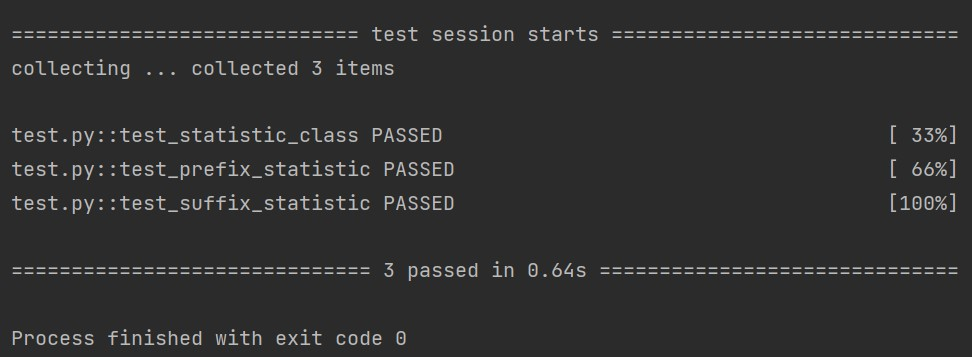
\includegraphics[scale= 0.7]{tests}
    \caption{Тестирование разработанного программного кода и структуры данных}
\end{figure}

\newpage
\section*{Заключение}
\addcontentsline{toc}{section}{Заключение}
	В результате производственной практики были достигнуты все поставленные цели и задачи. Разработанный модуль статистики префиксов предоставляет весь необходимый функционал для последующей генерации текстов на его основе. Благодаря созданию собственной C++ структуры данных на основе префиксного дерева (бора) из [1], разработанное решение является одним из оптимальных для алгоритма Маркова. 

      В ходе решении задач производственной практики были изучены и закреплены навыки подключения собственных структур данных на C/C++ в Python, создание модулей обёрток; модульное тестирование методов классов. Созданный в процессе производственной практики программный код, его тесты и документация доступы на  \href{https://github.com/Flexagen/Construction-of-suffix-and-prefix-statistics}{GitHub} для использования в дальнейших задачах.

\newpage
\addcontentsline{toc}{section}{Список литературы}
\begin{thebibliography}{}
	\bibitem{} {Керниrан, Брайан У., Пайк, Роб. Практика программирования. : Пер. с англ. - М. : ООО "И.Д. Вильямс", -288 с.}
\end{thebibliography}
\end{document}
